\documentclass{standalone}
\usepackage{tikz}
\begin{document}
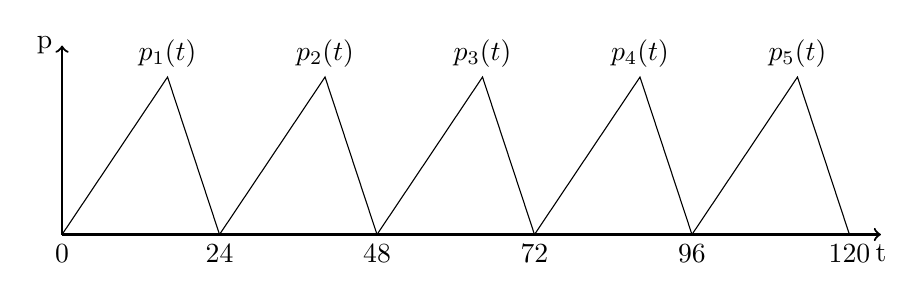
\begin{tikzpicture}[scale = 0.2]
\def\m{10.0}
\def\h{10.0}
\def\s{0.67}
\draw[->, thick] (0,0) -- (52, 0);
\draw[->, thick] (0,0) -- (0, 12);
\node [below, minimum size = 0.25cm] at (52,0) {t};
\node [left] at (0,12) {p};

\draw (0 * \m, 0) -- (0.67 * \m, \h) -- (\m, 0);
\draw (1 * \m, 0) -- (1.67*\m, \h) -- (2*\m,0);
\draw (2 * \m, 0) -- (2.67 * \m, \h) -- (3*\m,0);
\draw (3 * \m, 0) -- (3.67 * \m, \h) -- (4*\m,0);
\draw (4 * \m, 0) -- (4.67 * \m, \h) -- (5*\m,0);

\node [above] at (0.67 * \m, \h) {$p_1(t)$};
\node [above] at (1.67 * \m, \h) {$p_2(t)$};
\node [above] at (2.67 * \m, \h) {$p_3(t)$};
\node [above] at (3.67 * \m, \h) {$p_4(t)$};
\node [above] at (4.67 * \m, \h) {$p_5(t)$};

\node [below] at (0,0) {0};
\node [below] at (10,0) {24};
\node [below] at (20,0) {48};
\node [below] at (30,0) {72};
\node [below] at (40,0) {96};
\node [below] at (50,0) {120};
\end{tikzpicture}
\end{document}